\documentclass[xcolor=dvipsnames]{beamer}

\usepackage[utf8]{inputenc}
\usepackage{multicol}
\usepackage{amssymb,amsmath,amsbsy,cmath} 
\usepackage{bm}    
\usepackage{graphicx,graphics,xcolor}
\usepackage{xcolor}
\usepackage{physics}
\usepackage{comment}
\usepackage{caption}
\usepackage[style=authortitle,backend=bibtex]{biblatex}
\addbibresource{References.bib}
\usepackage{yfonts}
\usepackage{pifont}


\newcommand\blfootnote[1]{%
  \begingroup
  \renewcommand\thefootnote{}\footcite{#1}%
  \addtocounter{footnote}{-1}%
  \endgroup
}


\usetheme{Madrid}
\useoutertheme{miniframes} % Alternatively: miniframes, infolines, split
\useinnertheme{circles}


\title[Schwartzschild geometry]{Schwartzschild Geometry: Geodesics for massless particles}
\date{\today}
\author[Universidad del Valle]{ Juan E. Bedoya }
\institute[]{Universidad del Valle \\ Departamento de física}

\begin{document}
	
	\begin{frame}
		\titlepage
	\end{frame}
	
	\begin{frame}{Table of contents}
    \tableofcontents
	\end{frame}
	
	
	
	\section{Ecuaciones de movimiento en la métrica de Schwarzschild}
	\subsection{Métrica y ecuaciones generales}
	\begin{frame}{Métrica de Schwarzschild}
	    
	    \begin{block}{}
	   
	    \begin{equation*}
	    ds^{2}=c^{2}\Big( 1- \frac{2\mu}{r}\Big) dt^{2}-\Big( 1- \frac{2\mu}{r}\Big)^{-1} dx^{2}-r^{2}d\theta^{2}-r^{2}sen^{2}(\theta)d\phi^{2} 
	    \end{equation*}\\
	   Siendo $\mu=\frac{GM}{c^{2}}$
	\begin{equation*}
	\mathbb{G}=
     \begin{bmatrix}
      c^{2}\Big( 1- \frac{2\mu}{r}\Big) & 0&0&0\\
      0 &-\Big( 1- \frac{2\mu}{r}\Big)^{-1}&0&0\\
      0&0&-r^{2}&0\\
      0&0&0&-r^{2} sen^{2}(\theta)\\
\end{bmatrix}
\end{equation*}

  \end{block}

	\end{frame}
	
	
	\begin{frame}{Lagrangiano}
	    
	    \begin{block}{}
	   Sabemos que en relatividad el lagrangiano es de la forma
	    \begin{equation*}
	    L=g_{ab}\frac{dx^{a}}{d\sigma}\frac{dx^{b}}{d\sigma}
        \end{equation*}
       Lo que nos lleva a que:
	    \begin{equation*}
	    L=c^{2}\Big( 1-\frac{2\mu}{r} \Big)\dot{t}^{2}-\Big( 1-\frac{2\mu}{r} \Big)^{-1}\dot{r}^{2}-r^{2}\dot{\theta}^{2}-r^{2}sen^{2}(\theta)\dot{\phi}^{2}
        \end{equation*}       
       Siendo $\sigma$ un parámetro afín y además $\dot{x^{\mu}}=\frac{dx^{\mu}}{d\sigma}$. luego la ecuación de Euler-Lagrange para dicho parámetro es de la forma:
       \begin{equation*}
           \frac{d}{d\sigma}\Big(\frac{\partial L}{\partial \dot{x}^{\mu}} \Big)-\frac{\partial L}{\partial X^{\mu}}=0
       \end{equation*}
  \end{block}
	\end{frame}
	
	
	\begin{frame}{Ecuaciones de movimiento}
	    
	    \begin{block}{}
	    \begin{eqnarray}
      \Big(1-\frac{2\mu}{r} \Big)\dot{t}&=&k \label{0}\\
      \frac{\ddot{r}}{\Big(1-\frac{2\mu}{r} \Big)}-\frac{\mu\dot{r}^{2}}{\Big(1-\frac{2\mu}{r} \Big)^{2} r^{2}}+\frac{c^{2}\mu}{r^{2}}\dot{t}^{2}-r(\dot{\theta}^{2}+sen^{2}(\theta)\dot{\phi}^{2})&=&0 \label{1}\\
      \ddot{\theta}+\frac{2}{r}\dot{r}\dot{\theta}-sen(\theta)cos(\theta)\dot{\phi}^{2}&=&0 \label{2}\\
      r^{2}sen^{2}(\theta)\dot{\phi}&=&h\label{3}
        \end{eqnarray}\\
        
    Si $\theta=\frac{\pi}{2}$. la ecuación de $\theta$ se reduce a una geodésica usual, lo que nos permite aprovecharnos de la "simetría esférica" de la métrica.
        \end{block}
        \end{frame}
	
	
	\begin{frame}{interpretaciones de la constantes $h$ y $k$}
	    
	    \begin{block}{}
     Por analogía a las ecuaciones de Lagrange usuales se tiene que el 4-momento es de la forma
	    \begin{eqnarray*}
	    p_{\mu}=\frac{\partial L}{\partial \dot{x}^{\mu}}
        \end{eqnarray*}
        Es evidente por L que tanto $p_{0}$ como $p_{3}$ se conservan.\\ Por otro lado, si se elige un parámetro afín tal que $p^{\mu}=\dot{x}^{\mu}$ y además se usan las ecuaciones halladas con el lagrangiano  se llega a que: 
        \begin{eqnarray*}
	    p_{0}&=&\dot{x}_{0}=g_{00}\dot{x}^{0}= c^2\Big(1-\frac{2\mu}{r} \Big)\dot{t}=\overbrace{c^{2}k}^{Ecua. \ref{0}}\\
	    p_{3}&=&\dot{x}_{3}=g_{33}\dot{x}^{3}=-r^{2}\dot{\phi}=\underbrace{-h}_{ecua.\ref{3}}
        \end{eqnarray*}\\
        \end{block}
        \end{frame}
	
	
	\begin{frame}{Valores de $k$ y la energía}
	    
	    \begin{block}{}
    Finalmente, se conoce la energía de una partícula con un 4-momento $\textbf{p}$ que es vita por un observador con una 4-velocidad $\textbf{u}$ es de la forma
	    \begin{eqnarray*}
	    E=\textbf{u}\cdot \textbf{p}=p_{\mu} u^{\mu}\\
        \end{eqnarray*}\\
        Si $\textbf{u}=(1,0,0,0)$, entonces
        \begin{eqnarray*}
	    E&=&p_{0}\\
	    E&=&c^{2}k\\
	    \frac{E}{c^{2}}&=&k\\
        \end{eqnarray*}\\
        \end{block}
        \end{frame}


\subsection{Ecuaciones de movimiento para fotones}	


  \begin{frame}{Ecuaciones básicas para fotones}
    \begin{block}{}
        Volviendo a las ecuaciones de movimiento previas, y realizando las consideraciones mencionadas se llega a que:
          \begin{eqnarray}
      \Big(1-\frac{2\mu}{r} \Big)\dot{t}&=&k \label{02}\\
      \frac{\ddot{r}}{\Big(1-\frac{2\mu}{r} \Big)}-\frac{\mu\dot{r}^{2}}{\Big(1-\frac{2\mu}{r} \Big)^{2} r^{2}}+\frac{c^{2}\mu}{r^{2}}\dot{t}^{2}-r\dot{\phi}^{2}&=&0 \label{12}\\
      r^{2}\dot{\phi}&=&h\label{22}
        \end{eqnarray}\\
\end{block}
    
    \begin{block}{}
        Pero la ecuación \ref{12}, se puede reemplazar por su primera integral que es de la forma
        \begin{eqnarray}
      g_{\mu \nu}\dot{x}^{\mu}\dot{x}^{\nu}&=&0
        \end{eqnarray}\\
    \end{block}
  \end{frame}


  \begin{frame}{Ecuaciones finales para fotones}
    \begin{block}{}
        Volviendo a las ecuaciones de movimiento previas, y realizando las consideraciones mencionadas se llega a que:
          \begin{eqnarray}
      \Big(1-\frac{2\mu}{r} \Big)\dot{t}&=&k \label{02}\\
      c^{2}\Big( 1- \frac{2\mu}{r}\Big) \dot{t}^{2}-\Big( 1- \frac{2\mu}{r}\Big)^{-1} \dot{r}^{2}-r^{2}\dot{\phi}^{2}&=&0\label{1f} \\
       r^{2}\dot{\phi}&=&h\label{2f}
        \end{eqnarray}\\
    \end{block}
  \end{frame}

  \begin{frame}{Ecuación radial}
    \begin{block}{}
    si se unifican todas las ecuaciones de movimiento en la ecuación radial se tiene que:
          \begin{eqnarray*}
      c^{2}\Big( 1- \frac{2\mu}{r}\Big) \dot{t}^{2}-\Big( 1- \frac{2\mu}{r}\Big)^{-1} \dot{r}^{2}-r^{2}\dot{\phi}^{2}&=&0\\
      c^{2}\overbrace{\Big( 1- \frac{2\mu}{r}\Big)^{2} \dot{t}^{2}}^{k^{2}}- \dot{r}^{2}-\overbrace{r^{2}\dot{\phi}^{2}}^{h^2/r^{2}}\Big( 1- \frac{2\mu}{r}\Big)&=&0\\
      \dot{r}^{2}+\frac{h^2}{r^{2}}\Big( 1- \frac{2\mu}{r}\Big)&=& c^{2}k^{2}
        \end{eqnarray*}\\
    \end{block}
  \end{frame}
  
  
  \begin{frame}{}
    \begin{block}{}
    Luego, se tiene que
          \begin{eqnarray*}
          \frac{dr}{d\sigma}&=&\frac{dr}{d\phi}\overbrace{\frac{d\phi}{d\sigma}}^{\dot{\phi}=h/r^{2}}=\frac{dr}{d\phi}\frac{h}{r^{2}}
        \end{eqnarray*}\\
    \end{block}
    \begin{block}{}
    Entonces
    \begin{eqnarray*}
    \Big(\frac{dr}{d\phi}\frac{h}{r^{2}}\Big)^{2}+\frac{h^2}{r^{2}}\Big( 1- \frac{2\mu}{r}\Big)&=& c^{2}k^{2}\\
    \Big(\frac{dr}{d\phi}\frac{1}{r^{2}}\Big)^{2}+\frac{1}{r^{2}}\Big( 1- \frac{2\mu}{r}\Big)&=&\frac{c^{2}k^{2}}{h^{2}} \\
    \end{eqnarray*}\\
    \end{block}
    
  \end{frame}
  
  
    \begin{frame}{}
    \begin{block}{}
    Por otro lado, se define $u=1/r$, entonces
          \begin{eqnarray*}
          \frac{du}{d\phi}&=&-\frac{1}{r^{2}}\frac{dr}{d\phi}\\
          -\frac{1}{u^{2}}\frac{du}{d\phi}&=&\frac{dr}{d\phi}
        \end{eqnarray*}\\
    \end{block}
    \begin{block}{}
    Volviendo a la ecuación radial y aplicando el cambio de variable u se llega a que
    \begin{eqnarray*}
    \Big(\frac{dr}{d\phi}\frac{1}{r^{2}}\Big)^{2}+\frac{1}{r^{2}}\Big( 1- \frac{2\mu}{r}\Big)&=&\frac{c^{2}k^{2}}{h^{2}} \\
    \Big(-\frac{u}{d\phi}\frac{u^{2}}{u^{2}}\Big)^{2}+u^{2}\Big( 1- 2u\mu\Big)&=&\frac{c^{2}k^{2}}{h^{2}} \\
    \Big(\frac{du}{d\phi}\Big)^{2}+u^{2}- 2u^{3}\mu&=&\frac{c^{2}k^{2}}{h^{2}} 
    \end{eqnarray*}\\    
    \end{block}
  \end{frame}


    \begin{frame}{Ecuación radial}
    \begin{block}{}
    Finalmente, la ecuación radial queda de la forma
          \begin{eqnarray*}
    \Big(\frac{du}{d\phi}\Big)^{2}+u^{2}-2u^{3}\mu&=&\frac{c^{2}k^{2}}{h^{2}} \\
    2\frac{du}{d\phi}\frac{d^{2}u}{d\phi^{2}}+2u\frac{du}{d\phi}-6u^{2}\frac{du}{d\phi}\mu&=&0\\
    \frac{d^{2}u}{d\phi^{2}}+2u-3u^{2}\mu&=&0 \\
    \frac{d^{2}u}{d\phi^{2}}+2u-\frac{3GM}{c^{2}}u^{2}&=&0    
    \end{eqnarray*}\\    
    \end{block}
  \end{frame}
  

    \begin{frame}{Soluciones a la ecuación radial}
\begin{figure}
    \centering
    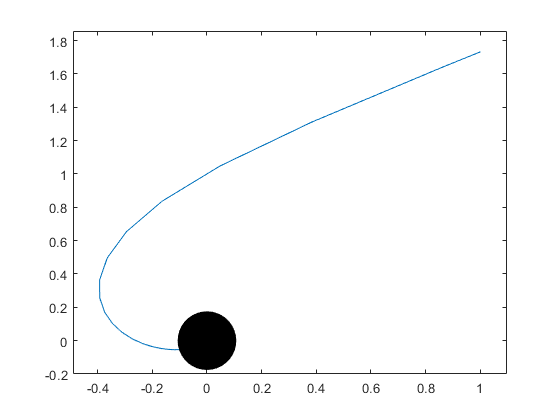
\includegraphics[width=0.75\textwidth]{Presentations/Images/3_foton_en.png}
\end{figure}
  \end{frame}


    \begin{frame}{Soluciones a la ecuación radial}
\begin{figure}
    \centering
    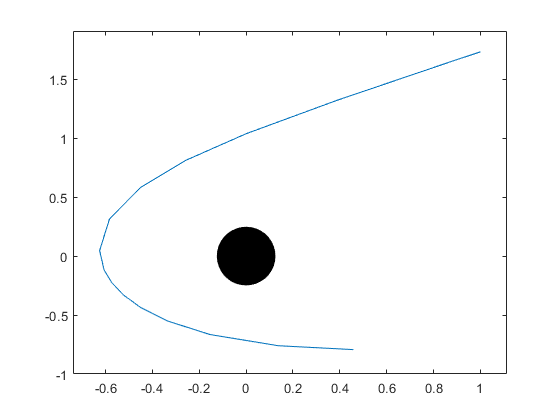
\includegraphics[width=0.75\textwidth]{Presentations/Images/3_foton_esc.png}
\end{figure}
  \end{frame}



\section{Casos especiales de la ecuaciónde movimento}
  \subsection{Movimiento radial}
    \begin{frame}{Movimiento radial ($\dot{\phi}=0$)}
    \begin{block}{}
     Si volvemos a las ecuaciones finales de movimiento y vemos la ecuación radial para $\dot{\phi}=0$ se llega a que:
  \begin{eqnarray*}
       c^{2}\Big( 1- \frac{2\mu}{r}\Big) \dot{t}^{2}-\Big( 1- \frac{2\mu}{r}\Big)^{-1} \dot{r}^{2}&=&0\\
       \pm  c\Big( 1- \frac{2\mu}{r}\Big)&=&\frac{dr}{dt}
 \end{eqnarray*}
      \end{block}
      \begin{block}{}
    Cuya solución es:
  \begin{eqnarray*}
       ct=\pm r\pm Ln\Big| \frac{r}{2\mu}-1 \Big|\\
 \end{eqnarray*}
 siendo + para los fotones saliendo y - para los fotones entrando
      \end{block}
  \end{frame}


\begin{frame}{}

     
      \begin{block}{Solución para movimiento radial}
  \begin{eqnarray*}
       ct=\pm r\pm Ln\Big| \frac{r}{2\mu}-1 \Big|\\
 \end{eqnarray*}
 
   \end{block}
    \begin{block}{casos limite}
    \begin{itemize}
        \item Si $t=-t$ $\Rightarrow$ Las trayectorias salientes se comvierten en entrates y viceversa.
        \item Si $r\rightarrow \infty$ $\Rightarrow$ El termino de r va a dominar sobre el del logaritmo llegando a que $ct=r$ los que no lleva a la relatividad especial.
        \item Si $r\rightarrow 2\mu$ $\Rightarrow$ el logaritmo se va a infinito, luego $ct\rightarrow \pm \infty$, mientras mas nos acerquemos a $2\mu$ el cono de luz es mas vertical 
    \end{itemize}
      \end{block}
  \end{frame}



    \begin{frame}{}
\begin{figure}
    \centering
    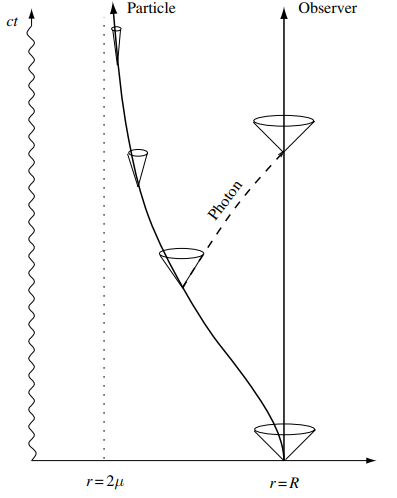
\includegraphics[width=0.5\textwidth]{Presentations/Images/3_foton_radia.png}
\end{figure}
  \end{frame}


\subsection{Movimiento Cicular}
\begin{frame}{Movimiento Circular $(\dot{r}=0)$}
    \begin{block}{}
    Si imponemos la condición  $\dot{r}=0$ en la ecuación radial se obtiene que
    \begin{eqnarray*}
          R=\frac{3GM}{c^{2}}\approx 4.5 Km
    \end{eqnarray*}
    este fenomeno es inestable (luego veremos porque) y además el radio es muy pequeño.\\
    
    \end{block}
\end{frame}


\subsection{Estabilidad de las orbitas}
\begin{frame}{Estabilidad de las orbitas}
    \begin{block}{}
    Si se vuleve a la ecuación radial antes del cambio a u se obtiene que
    \begin{eqnarray*}
      \frac{1}{h^{2}}\dot{r}^{2}+\overbrace{\frac{1}{r^{2}}\Big( 1- \frac{2\mu}{r}\Big)}^{V_{eff}}&=& \overbrace{c^{2}k^{2}/h^{2}}^{1/b^{2}}\\
    \end{eqnarray*}
    si se renormaliza el parametro afín tal que $\sigma=h\sigma$ se llega a que
    \begin{eqnarray*}
      \dot{r}^{2}+V_{eff}&=& \frac{1}{b^{2}}\\
    \end{eqnarray*}
    \end{block}
\end{frame}


\begin{frame}{Inestabilidad de las orbitas y el potencial}
    \begin{figure}
        \centering
        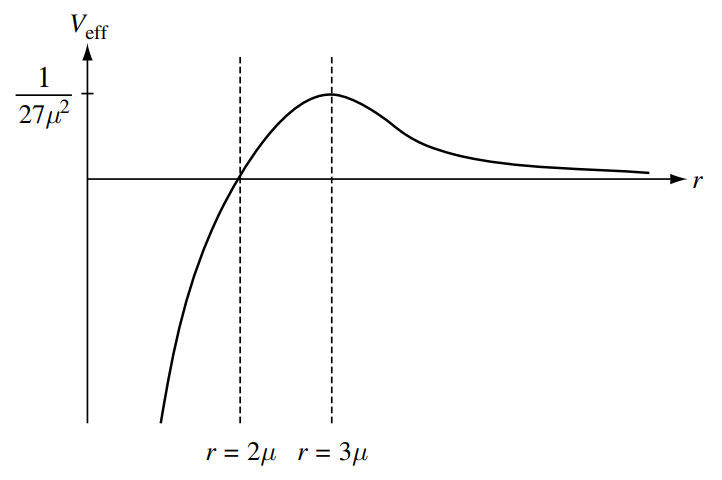
\includegraphics[width=0.8\textwidth]{Presentations/Images/3_poten.png}
    \end{figure}
\end{frame}


\begin{frame}{Definición del parametro b}
    \begin{block}{}
    Usando la ecuación radial antes del cambio a u se llega a que
    \begin{eqnarray*}
    \frac{d\phi}{dr}&=&\pm \frac{1}{r^{2}}\Big[ \frac{1}{b^{2}} -\frac{1}{r^{2}}\Big(1-\frac{2\mu}{r} \Big) \Big]^{-1/2}
    \end{eqnarray*}
    si $r \rightarrow \infty$
    \begin{eqnarray*}
    \frac{d\phi}{dr}&=&\pm \frac{1}{r^{2}}b\\
    \end{eqnarray*}
    \end{block}
\end{frame}


\end{document}






